% !TEX TS-program = pdflatex
% !TEX encoding = UTF-8 Unicode

% This is a simple template for a LaTeX document using the "article" class.
% See "book", "report", "letter" for other types of document.

\documentclass[11pt]{article} % use larger type; default would be 10pt


\usepackage{ulem}
\newcommand\NoIndent[1]{%
  \par\vbox{\parbox[t]{\linewidth}{#1}}%
}


\usepackage[utf8]{inputenc} % set input encoding (not needed with XeLaTeX)

%%% Examples of Article customizations
% These packages are optional, depending whether you want the features they provide.
% See the LaTeX Companion or other references for full information.

%%% PAGE DIMENSIONS
\usepackage{geometry} % to change the page dimensions
\geometry{a4paper} % or letterpaper (US) or a5paper or....
% \geometry{margin=2in} % for example, change the margins to 2 inches all round
% \geometry{landscape} % set up the page for landscape
%   read geometry.pdf for detailed page layout information

\usepackage{graphicx} % support the \includegraphics command and options

% \usepackage[parfill]{parskip} % Activate to begin paragraphs with an empty line rather than an indent

%%% PACKAGES
\usepackage{booktabs} % for much better looking tables
\usepackage{array} % for better arrays (eg matrices) in maths
\usepackage{paralist} % very flexible & customisable lists (eg. enumerate/itemize, etc.)
\usepackage{verbatim} % adds environment for commenting out blocks of text & for better verbatim
\usepackage{subfig} % make it possible to include more than one captioned figure/table in a single float
% These packages are all incorporated in the memoir class to one degree or another...

%%% HEADERS & FOOTERS
\usepackage{fancyhdr} % This should be set AFTER setting up the page geometry
\pagestyle{fancy} % options: empty , plain , fancy
\renewcommand{\headrulewidth}{0pt} % customise the layout...
\lhead{}\chead{}\rhead{}
\lfoot{}\cfoot{\thepage}\rfoot{}

%%% SECTION TITLE APPEARANCE
\usepackage{sectsty}
\allsectionsfont{\sffamily\mdseries\upshape} % (See the fntguide.pdf for font help)
% (This matches ConTeXt defaults)

%%% ToC (table of contents) APPEARANCE
\usepackage[nottoc,notlof,notlot]{tocbibind} % Put the bibliography in the ToC
\usepackage[titles,subfigure]{tocloft} % Alter the style of the Table of Contents
\renewcommand{\cftsecfont}{\rmfamily\mdseries\upshape}
\renewcommand{\cftsecpagefont}{\rmfamily\mdseries\upshape} % No bold!

%%% END Article customizations


\usepackage{verbatim}
\usepackage{amsmath}


\title{Work Log for September}
\author{Logan Brown}
%\date{} % Activate to display a given date or no date (if empty),
         % otherwise the current date is printed 

\begin{document}
\maketitle
%\tableofcontents


\setcounter{section}{3} %week number minus 1
\setcounter{subsection}{-1}
\setcounter{subsubsection}{0}

\section{Week of September 22nd-26th}
\subsection{Goals for the Week}
\begin{enumerate}
\item Write out the math from 9/19 (from the green notebook)
\item Get observed yeast phi values from REU data
\item Run NSE model with the Browser line when $phi$ is proposed to see what is causing NaN
\item Ideally, an NSE patch to fix it (try NaN to NA?)
\item Disect NSE data structure
\end{enumerate}

\subsection{Progress/Notes}

\subsubsection{Write out the math from 9/19 (from the green notebook)}

see genomeProb.tex and genomeProb.pdf

\subsubsection{Get observed yeast phi values from REU data}

\subsubsection{Run NSE model with the Browser line when $phi$ is proposed to see what is causing NaN}

7/22: The local library has been built. I removed the \& to ensure that browser() will activate, and and wrote in two checks in my.logdmultinomCodOne.r

\verbatiminput{misc/browsercommand.txt}

but it's taken nearly 8 hours to run!!! The run started at: 2014-09-22 10:24:55 

I left at 18:15:, so I don't know what happens.

The run finished at 18:28. But... browser didn't launch? I think I'll have to go into R manually, and use

\verbatiminput{misc/browsercommand2.txt}

This means I'll have to parse the command line arguments manually.


CAUGHT

\verbatiminput{misc/errorlogs.txt}

This means that it's actually not catching in my.logdmultinomCodOne.r

It catches in my.drawPhiConditionalAll. \sout{but lpProp comes from my.logPosteriorAll.lognormal\_bias. Which comes from} .cubfitsEnv does not correctly get MY functions. So it never got my.lodgmultinomCodOne with the browser() commands. Interesting.

I've done two separate runs of nsef cubfits.

\begin{enumerate}
\item one of the elements of lpProp is going to NaN.
\item It is not always the same element. For my first run, it was zraS. The second was ecnA.
\item It is not because log(0)$= -\infty$. Multiple elements are going to -Inf (106 in the first run,  87 in the second run). Moreover, the roc code also tends to generate -Inf values (though not nearly as many in each run, only 1 or 2).
\item It doesn't appear that the scale is going out of control. Scale and acceptance rate stay similar to the values used in the ROC model.
\item It happens in cubfits and cubappr 
\item It is not just happening for one amino acid. For the first run, it happened in Amino Acid 5 (F). In the run, it happened in both 8 and 9 (I and K). The third run happened in 11 (N).
\item It is lp.vec, the return from my.inverse.mlogit.r

\item All the values for lpProp are generally too low.\\
mean(lpProp[is.finite(lpProp)]) returns -588.3597 in from the first run, and -554.7103 in the second run.\\

Taking that out of the log scale (using mean( exp(lpProp[is.finite(lpProp)]) ) instead) gives 1.10973e-11 for the first and 1.085067e-12 for the second.

%Below, I've graphed the middle 80\% of the lpProp values. plot(sort(exp(lpProp))[225:2025])

%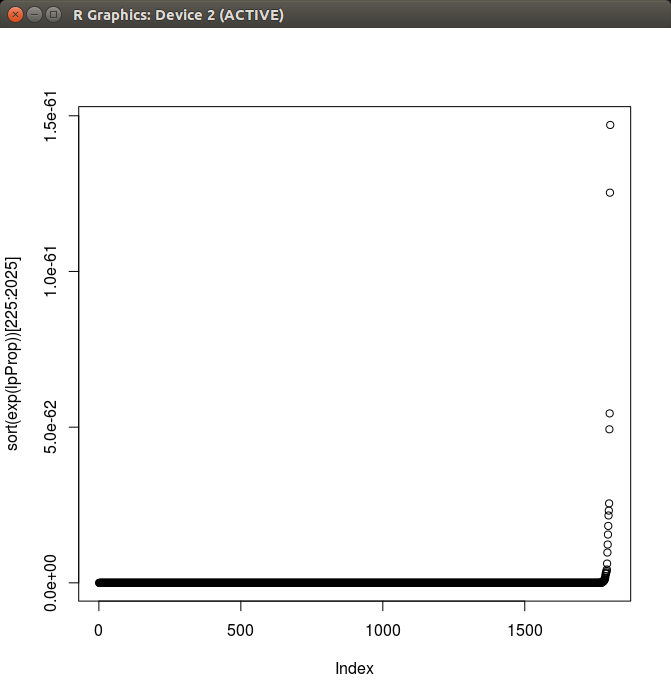
\includegraphics[width=\textwidth]{data/middle80percent1.png}
%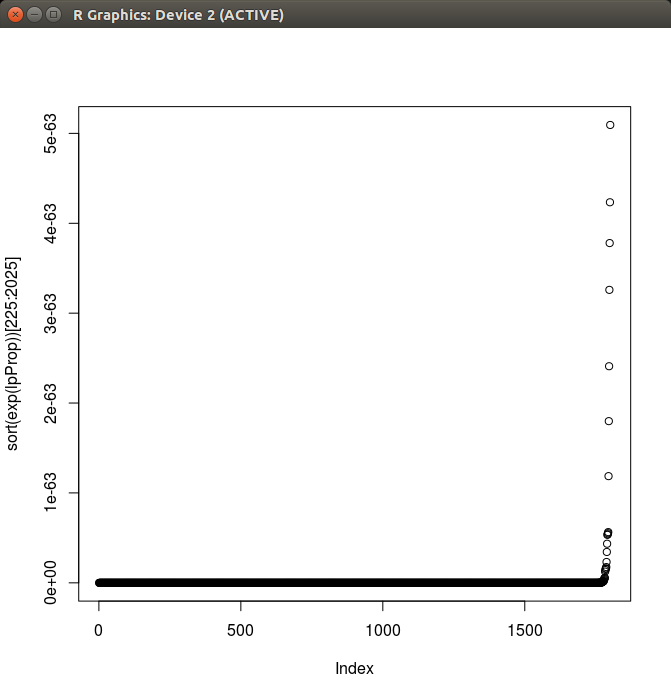
\includegraphics[width=\textwidth]{data/middle80percent2.png}

Below is the information on a log scale. Note that while the probabilities were initially also on a log scale, they have been exponentiated. Also, note that the information doesn't actually follow any kind of a trend. I sorted the data in order to take off the top and bottom 10\%.

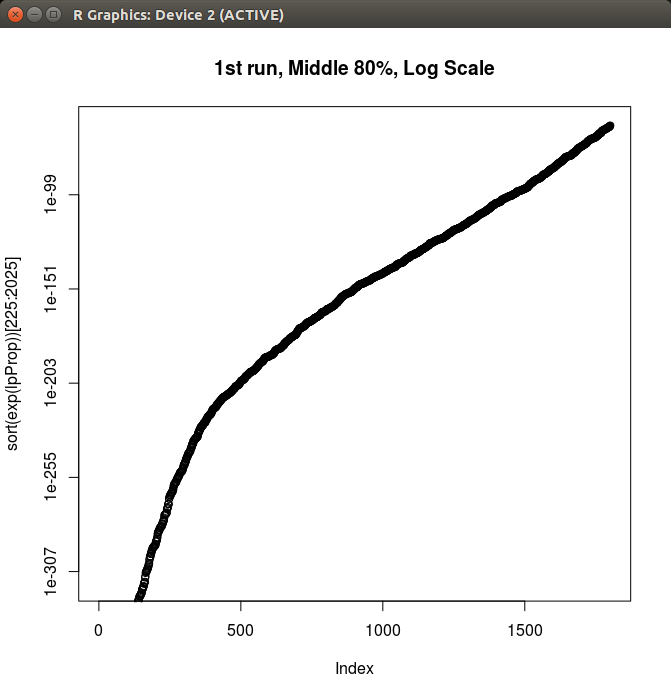
\includegraphics[width=0.5\textwidth]{data/middle80log1.png}
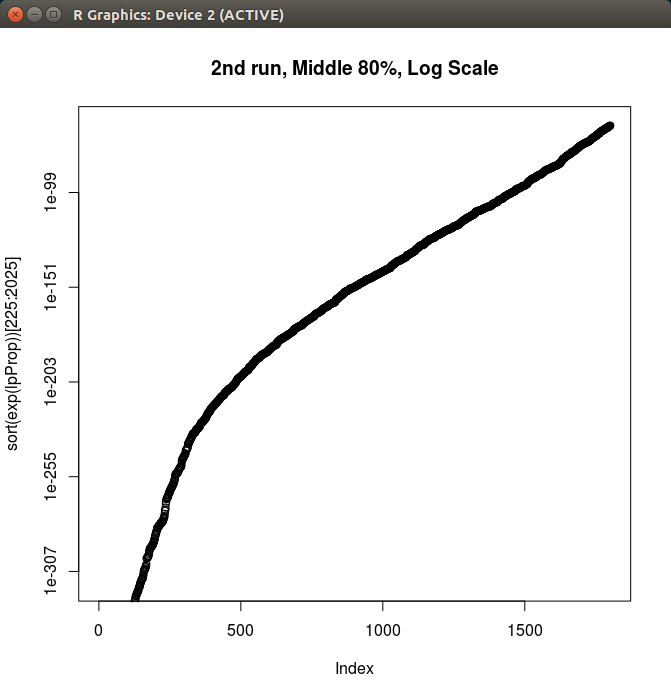
\includegraphics[width=0.5\textwidth]{data/middle80log2.png}

Unfortunately that's all the information I was able to get because the terminal crashed. 

Rerunning using GDB on R. When I hit the browser (when lpProp has NaN), I should be able to launch the C code using GDB and find EXACTLY the error.

\end{enumerate}







\subsubsection{Ideally, an NSE patch to fix it (try NaN to NA?)}

\subsubsection{Disect NSE Data Structure}

Position information? is in reu13.df\$(amino acid)\$Pos

\subsubsection{Rstudio / R vim extension?}

\subsubsection{Reread Debugging Chapter}




\subsection{Goals for next Week}
\begin{enumerate}
\item Future Goal
\end{enumerate}


\end{document} %End of day document, REMOVE
